\subsection{Esecuzione dell'esperienza}

L'esecuzione dell'esperienza è molto semplice. Avevamo a nostra disposizione le seguenti diapositive:

\begin{itemize}
    \item{Diapositiva con fessure di larghezza nominale 160, 80, 40 e 20 micrometri.}
    \item{Diapositiva con 5 fili di spessore sconosciuto a cui abbiamo aggiunto un capello di uno dei membri del gruppo.}
    \item{Diapositiva con 2 fori di diametro ignoto.}
    \item{Diapositiva con 3 reticoli da 100, 300 e 600 fessure per millimetro.}
\end{itemize}

\begin{figure}[b!]
    \centering
    \begin{subfigure}[b]{0.3\textwidth}
        \includegraphics[width=\textwidth]{f1.png}
        \caption{Filo o fessura}
        \label{fig:ff}
    \end{subfigure}%
    ~ %add desired spacing between images, e. g. ~, \quad, \qquad etc.
      %(or a blank line to force the subfigure onto a new line)
    \begin{subfigure}[b]{0.3\textwidth}
        \includegraphics[width=\textwidth]{f2.png}
        \caption{Foro}
        \label{fig:foro}
    \end{subfigure}
    ~ %add desired spacing between images, e. g. ~, \quad, \qquad etc.
      %(or a blank line to force the subfigure onto a new line)
    \begin{subfigure}[b]{0.3\textwidth}
        \includegraphics[width=\textwidth]{f3.png}
        \caption{Reticolo}
        \label{fig:ret}
    \end{subfigure}
    \caption{Figure di diffrazione generate da diversi tipi di ostacoli. Notare che, in maniera contro intuitiva,
        le aree nere sono quelle illuminate, mentre quelle bianche sono quelle che restano al buio.}
    \label{fig:diff}
\end{figure}

Le misure sono state eseguite nel seguente modo. Per ogni diapositiva, abbiamo posto sul percorso del raggio laser ogniuno degli ostacoli
presenti sulla diapositiva, uno alla volta (ovviamente :-) ). Nel fare ciò, ci siamo presi la briga di controllare, alzando ed abbassando
la diapositiva, che la figura di diffrazione fosse la più pulita possibile. Questo significa trovare il luogo della fessura che ha i bordi
migliori. Dopodiché abbiamo incollato allo schermo una striscia di carta per annotare picchi di luce ed ombra. La distanza tra le tacche
è stata misurata con il calibro. Siccome la figura cambia a seconda dell'ostacolo abbiamo variato la procedura di misura come segue:

\begin{itemize}
    \item{Nel caso di fili e fessure la figura di diffrazione è lineare e presenta dei massimi e minimi larghi e ``sfuocati'' con un andamento
        sinusoidale (si veda Figura \ref{fig:ff}). Abbiamo segnato sulla carta i minimi di intensità, ovvero le parti dello schermo
        che restano al buio.}
    \item{Nel caso dei fori la figura di diffrazione è un cerchio centrale con vari anelli luminosi concentrici separati da
        zone scure (minimi di intensità, si veda Figura \ref{fig:foro}). Inoltre, a parte il centro ed il primo anello,
        la figura è molto debole e difficilmente
        percepibile ad occhio nudo. Poiché la misura del primo minimo è difficoltosa a causa della larghezza dello stesso, abbiamo segnato
        l'inizio e la fine del minimo e poi mediato i valori ottenuti.}
    \item{Nel caso dei reticoli di diffrazione la figura di interferenza presenta dei picchi molto luminosi e dei minimi molto larghi
            (In realtà ci sono anche dei minimi secondari, ma sono talmente deboli da non essere percepibili. Disegno in Figura \ref{fig:ret}).
            La misura dei minimi è quindi esclusa, per cui abbiamo misurato la separazione tra i massimi dello stesso ordine.}
\end{itemize}

Le Tabelle \ref{tab:ff} e \ref{tab:foret} riportano tutti i dati misurati. Ci teniamo a far notare
che, sebbene molte misure siano state effettuate con il calibro e siano riportate anche le frazioni di millimetro,
l'incertezza di queste misure è molto più alta, a causa dello spessore delle tacche segnate sul foglio e a causa del
fatto che spesso erano storte e magari doppie. A nostro parere l'incertezza più appropiata sarebbe un incertezza di
risoluzione di 1 mm, che comunque non influisce in maniera significativa sui valori ottenuti dai calcoli.

\begin{table}[t!]
    \centering
    \footnotesize
    \begin{tabular}{l l l l | l l l l l l}
        \toprule
        \multicolumn{4}{c|}{Fessure [mm]} & \multicolumn{6}{c}{Fili [mm]}  \\
        160 um&    80 um&    40 um&    20 um&  Filo 1&  Filo 2&  Filo 3& Filo 4& Filo 5& Capello \\
        \midrule
        12.65&     24.80&    48.40&   103.30& 34.50&    21.35&   17.50&  10.65&  3.05&   28.55  \\
        25.50&     49.25&    97.10&   209.80& 70.70&    42.15&   34.20&  21.15&  8.30&   56.00  \\
        37.75&     73.70&   146.75&   313.00& 104.60&   62.45&   51.40&  30.30&  14.00&  84.15  \\
        50.10&     98.90&   195.00&         & 149.20&   82.45&   67.90&  40.70&  21.10&  112.40 \\
        62.55&    124.10&   246.05&         & 174.95&   104.15&  85.30&  50.75&  28.00&  139.15 \\
        74.85&    148.40&&                  & 124.30&   101.90&  60.85&  34.40&       &         \\      
        88.25&&&                            & 144.90&   118.30&  71.00&  41.60&       &         \\
        100.15&&&                           &       &   135.65&  81.00&  48.25&       &         \\
        113.10&&&                           &       &        &       &   54.55&       &         \\
        125.70&&&                           &       &        &       &        &       &         \\
        \bottomrule
    \end{tabular}
    \caption{Distanza misurata tra i minimi dello stesso ordine nel caso della diapositiva con le fessure ed
        in quella con i fili. Il titolo delle colonne, nel caso delle fessure, si riferisce alla larghezza nominale delle fessure.
        Tutte le misure sono riportate in millimetri e sono state misurate con il calibro ventesimale. Tuttavia
        le cifre dopo la virgola sono molto incerte a causa della dimensione delle tacche sulla carta, e non dovrebbero
        essere considerate significative.}
    \label{tab:ff}
\end{table}

\begin{table}[b!]
    \centering
    \footnotesize
    \begin{tabular}{l l | l l l | l l l}
        \toprule
        \multicolumn{2}{c|}{Fori [mm]} & \multicolumn{6}{c}{Reticoli [mm]} \\
        Foro 1 &      Foro 2 & R 100 &   R 300 &   R 600 & A 100 & A 300 & A 600\\
        \midrule
        63.50 &           32.75      & 198   &   597   &   1282  & 191   & 576   & 1232 \\
        65.00 &           30.25      & 399   &   1266  &         & 385   & 1218  &      \\
        64.00 &           29.50      & 640   &         &         & 584   &       &      \\
        63.50 &           30.00      &       &         &         &       &       &      \\
        \bottomrule
    \end{tabular}
    \caption{La tabella riporta i dati misurati per le diapositive con i fori e con i reticoli.
        Nel caso dei fori la figura di diffrazione è del tipo riportato in Figura \ref{fig:foro}
        ed i valori riportati sono alcuni diametri del primo minimo. Ogni valore è stato ottenuto mediando
        due dati misurati nel bordo interno e nel bordo esterno del minimo, poiché la misura diretta è risultata
        troppo arbitraria. Le misure sono state effettuate col calibro, ma le cifre dopo la virgola sono poco significative.
        I dati dei reticoli si riferiscono invece ai massimi di ordine uguale
        (primo ordine per la prima riga, secondo per la successiva, etc), poiché i minimi sono molto larghi.
        Le misure sono state effettuate colo metro poiché le distanze sono molto grandi. Nel titolo delle colonne R indica il laser
        rosso, A quello arancione, mentre il numero indica la densità di fessure per millimetro del reticolo. Le misure
        sono state effettuare per ogni reticolo con entrambi i laser. Tutte le misure sono in millimetri.}
    \label{tab:foret}
\end{table}

\subsection{Analisi dati}

L'analisi dati è divisa in 3 parti. Nella prima ci occupiamo di ottenere la dimensione degli ostacoli
che abbiamo messo sul percorso del raggio laser. La seconda si occupa di determinare la dimensione
delle fessure dei reticoli, prendendo come dato in input la lunghezza d'onda del laser usato.
La procedura da usare per ricavare la dimensione di fenditure, fili e fori è differente da quella usata
per i reticoli, per motivi che chiariremo in seguito.
Nella terza parte ci proponiamo di rovesciare la situazione: vogliamo calcolare la lunghezza d'onda dei due
laser usati prendendo come input la dimensione delle fessure dei reticoli, riportate sugli stessi dal costruttore.

\begin{wrapfigure}{r}{52mm}
    \vspace{-5mm}
    \begin{center}
        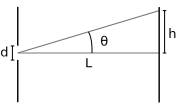
\includegraphics[width=48mm]{fen.pdf}
    \end{center}
    \vspace{-2mm}
\end{wrapfigure}

\subsubsection{Ostacoli vari}

Vogliamo calcolare la dimensione delle fenditure, dei fili e dei fori in esame.
La formula usata nell'analisi dati è la seguente:

\begin{equation}
    d = \frac{m\lambda}{\sin(\vartheta)}
    \label{eq:mindif}
\end{equation}

dove $d$ indica la larghezza della fenditura (si veda disegno a fianco),
$m \in \mathbb{Z} \setminus \{0\}$ indica l'ordine del minimo in questione,
$\lambda$ è la lunghezza d'onda della luce e $\vartheta$ è l'angolo che identifica
il minimo di ordine $m$ sullo schermo.

La formula si ottiene calcolando dove si trovano i minimi di intensità sullo schermo.
Quindi essa ci permette di ricavare $d$ se conosciamo la posizione di un qualsiasi minimo
della figura di diffrazione.

Durante l'esperimento abbiamo misurato la distanza tra minimi dello stesso ordine per i vari ostacoli.
Abbiamo quindi misurato la grandezza $2h$, i cui valori sono riportati nelle Tabelle \ref{tab:ff} e \ref{tab:foret}.
Nella (\ref{eq:mindif}) abbiamo bisogno di $\sin(\vartheta)$. Poiché gli angoli in gioco sono molto piccoli, tutti minori
di 6 gradi, possiamo usare l'approssimazione $\sin(\vartheta) \simeq \vartheta \simeq \tan(\vartheta)$. Inoltre abbiamo
misurato la distanza $L = \SI{1555}{\milli\metre}$ tra lo schermo e l'ostacolo.
Di conseguenza possiamo calcolare $\vartheta$ nel seguente modo:

\begin{equation}
    \tan(\vartheta) = \frac{h}{L}
\end{equation}

L'equazione (\ref{eq:mindif}) diventa quindi:

\begin{equation}
    d = \frac{m\lambda L}{h}
\end{equation}

\subsubsection{Reticoli}

\subsubsection{Lunghezza d'onda dei laser}
